% This is samplepaper.tex, a sample chapter demonstrating the
% LLNCS macro package for Springer Computer Science proceedings;
% Version 2.20 of 2017/10/04
%
\documentclass[runningheads]{llncs}
%
\usepackage{graphicx}

%%%%ДОБАВИЛ ДЛЯ РУССКОГО ТЕКСТА
\usepackage[utf8x]{inputenc}
\usepackage[english,russian]{babel}
\usepackage{cmap}
%%%%


% If you use the hyperref package, please uncomment the following line
% to display URLs in blue roman font according to Springer's eBook style:
% \renewcommand\UrlFont{\color{blue}\rmfamily}

\begin{document}
%
\title{Generalized dimensionality reduction scheme 
for global optimization problems
\thanks{This study was supported by the Russian Science Foundation, project 
No.\,16-11-10150.}}
%
\titlerunning{Generalized dimensionality reduction scheme}
% If the paper title is too long for the running head, you can set 
% an abbreviated paper title here
%
\author{Konstantin Barkalov %\orcidID{0000-0001-5273-2471}  
\and Ilia Lebedev %\orcidID{0000-0002-8736-0652}
}
%
\authorrunning{K. Barkalov, I. Lebedev}
% First names are abbreviated in the running head.
% If there are more than two authors, 'et al.' is used.
%
\institute{Lobachevsky State University of Nizhni Novgorod, Nizhni Novgorod, 
Russia \email{konstantin.barkalov@itmm.unn.ru}}
%
\maketitle              % typeset the header of the contribution
%
\begin{abstract}

В статье рассматриваются задачи многомерной многоэкстремальной оптимизации и численные методы их решения. Об оптимизируемой функции делается лишь общее предположение, что она удовлетворяет условию Липшица с неизвестной априори константой. Задачи такого типа часто встречаются в приложениях. 
Рассмотрено два подхода к редукции размерности в задачах многомерной оптимизации. Первый из них использует Peano-type space-filling curves, отображающие одномерный отрезок на многомерную область. Второй основан на nested optimization scheme, that reduces the mul- tidimensional problem to a family of one-dimensional subproblems.
Предложена обобщенная схема, комбинирующая эти два подхода. В новой схеме решение многомерной задачи сводится к решению семейства задач меньшей размерности, в которых, в свою очередь, используются space-filling curves. Реализован адаптивный алгоритм, в котором все возникающие подзадачи решаются одновременно. 
Проведены численные эксперименты на нескольких сотнях тестовых задач, подтверждающие эффективность предложенной обобщенной схемы.

\keywords{Global optimization \and Multiextremal functions \and 
Dimensionality reduction \and Peano curve \and Nested optimization \and 
Numerical methods.}
\end{abstract}
%
%
%
\section{Introduction}
This paper considers ''black-box'' global optimization problems of the following form:
\begin{eqnarray}\label{main_problem}
& \varphi(y^\ast)=\min{\left\{\varphi(y):y\in D\right\}},\\
& D=\left\{y\in R^N: a_i\leq y_i \leq b_i, 1\leq i \leq N\right\}. \nonumber
\end{eqnarray}
The objective function is assumed to satisfy the Lipschitz condition 
\[
\left|\varphi(y')-\varphi(y'')\right|\leq L\left\|y'-y''\right\|,\; y',y'' \in D,\; 0<L<\infty,
\]
with the constant $L$ unknown a priori.

\Russian
Известным способом решения многоэкстремальных задач являются мультистартовые схемы. В этих схемах в области поиска размещается некоторая сетка, точки которой использутся как стартовые поиска экстремума локальным методом, а затем выбирается наименьший из найденных экстремумов. Отдельной проблемой в рамках данного подхода является выбор стартовых точек, осуществляемый, как правило, на основе метода Монте-Карло \cite{Zhigljavsky2008}. Этот подход вполне применим для задач с небольшим числом локальных минимумов, имеющих широкие области притяжения, но для задач с существенной многоэкстремальностью его эффективность резко падает. 

В настоящее время для решения задач глобальной оптимизации широко используются генетические алгоритмы (см., например, \cite{Yang2013}), которые так или иначе основаны на идеях случайного поиска. В силу простоты реализации и использования они получили большую популярность, однако по качеству работы (численной оценкой которого может служить число корректно решенных задач из некоторого тестового набора) они существенно уступают детерминированным алгоритмам \cite{Kvasov2018,Sergeyev2018}.

Если говорить о детерминированных методах глобальной оптимизации, то многие методы данного класса основаны на различных способах разбиения области поиска на систему подобластей и последующего выбора наиболее перспективной подобласти для размещения очередного испытания (вычисления целевой функции). Результаты в данном направлении представлены в работах \cite{Zilinskas2010,Paulavicius2016,Evtushenko2013,Jones2009,Sergeyev2015}.

Наконец, для разработки методов многомерной оптимизации широко применяется подход, связанный с редукцией многомерной задачи к эквивалентной одномерной или системе одномерных подзадач и последующим решением одномерных задач эффективными методами оптимизации функций одной переменной. Используются две такие схемы: редукция на основе кривых, заполняющих пространство (кривых Пеано, или разверток) \cite{Strongin2000,Sergeyev2013}, и схема рекурсивной вложенной оптимизации \cite{Strongin2000,Grishagin2001}. В статье \cite{Grishagin2016} предложена адаптивная схема редукции, обобщающая классическую схему рекурсивной оптимизации. Адаптивная схема существенно повышает эффективность оптимизации по сравнению с базовым прототипом \cite{Grishagin2016_1}. В данной работе предлагается обобщение адаптивной схемы редукции размерности, комбинирующее использование вложенной оптимизации и кривых Пеано. При таком подходе вложенные подзадачи в адаптивной схеме могут быть как одномерными, так и многомерными. В последнем случае для редукции размерности вложенных подзадач используются развертки.


\section{The global search algorithm}
\label{SectionCore}

As a core problem we consider a one-dimensional multiextremal optimization 
problem
\begin{equation}\label{uni_problem}
\varphi^\ast = \varphi(x^\ast)=\min{\left\{\varphi(x):x\in \left[0,1\right] 
\right\}}
\end{equation}
with objective function satisfying the Lipschitz condition. 

Let us give the description of the global search algorithm (GSA) applied for 
solving the above problem (according to \cite{Strongin2000}). 
GSA involves constructing a sequence of points $x^i$, where the values of the 
objective function $z^i=\varphi(x^i)$ are calculated. Let us call the 
function value calculation process the \textit{trial}. 
According to the algorithm, the first two trials are executed at the ends of 
the interval  $[a,b]$, i.e., $x^0=a,\;x^1=b$. The function values $z^0=\varphi
(x^0),\;z^1=\varphi(x^1)$  are computed and the number $k$ is set to 1. In 
order to select the point of a new trial $x^{k+1}, k\geq 1,$  it is necessary 
to perform the following steps.

\textbf{Step 1.} Renumber by subscripts (beginning from zero) the points $x^i,
\:0\leq i\leq k$, of the previous trials in increasing order, i.e.,
\[
0=x_0<x_1<\ldots <x_{k}=1.
\] 
Juxtapose to the points $x_i, 0\leq i\leq k$,  the function values $z_i=
\varphi(x_i), 0\leq i\leq k$.

\textbf{Step 2.} Compute the maximum absolute value of the first divided 
differences 
\begin{equation}\label{mu}
\mu=\max_{1\leq i\leq k}\frac{\left|z_i-z_{i-1}\right|}{\Delta_i}
\end{equation}
where $\Delta_i = x_i-x_{i-1}$. If the above formula yields a zero value, 
assume that $\mu = 1$.

\textbf{Step 3.} For each interval $(x_{i-1},x_i),1\leq i\leq k$,  calculate 
the characteristic
\begin{equation}\label{R}
R(i)=r\mu\Delta_i+\frac{(z_i-z_{i-1})^2}{r\mu\Delta_i}-2(z_i+z_{i-1}),
\end{equation} 
where $r>1$ is a predefined parameter of the method. 

\textbf{Step 4.} Find the interval $(x_{t-1},x_t)$ with the maximum 
characteristic
\begin{equation}\label{MaxR}
R(t)=\max_{1\leq i\leq {k}}R(i).
\end{equation}  

\textbf{Step 5.} Execute the new trial at the point 
\begin{equation}\label{xk1}
x^{k+1}=\frac{1}{2}(x_{t-1}+x_t) - \frac{z_t-z_{t-1}}{2r\mu}.
\end{equation}

The algorithm terminates if the condition $\Delta_t<\epsilon$ is satisfied; 
here $t$ is from (\ref{MaxR}) and $\epsilon>0$ is the preset accuracy. For 
estimation of the global solution values
\[
z_k^\ast=\min_{0\leq i \leq k}\varphi(x^i), \ x_k^\ast=\arg \min_{0\leq i \leq
 k}\varphi(x^i).
\]
are selected. 
The theory of algorithm convergence is presented in \cite{Strongin2000}.

\section{Dimensionality reduction}
\subsection{Dimensionality reduction using Peano-type space-filling curves}
\label{SectionPeano}

The use of Peano curve $y(x)$ 
\begin{equation}
\left\{y\in R^N: -2^{-1}\leq y_i \leq 2^{-1}, 1 \leq i \leq N\right\}=\left\{
y(x):0\leq x \leq 1 \right\}
\end{equation}
unambiguously mapping the interval of real axis $[0,1]$ onto a 
$N$-dimensional cube is the first of the dimension reduction methods considered.
Problems of numerical construction of Peano-type space-filling curves and the 
corresponding theory are considered in detail in \cite{Strongin2000}, 
\cite{Sergeyev2013}. Here we will note that a numerically 
constructed curve (\textit{evolvent}) is $2^{-m}$ accurate approximation of 
the theoretical Peano curve, where $m$ is an evolvent construction parameter.

By using this kind of mapping it is possible to reduce the multidimensional 
problem~(\ref{main_problem}) to a univariate problem
\begin{equation}
\varphi(y^\ast)=\varphi(y(x^\ast))=\min{\left\{\varphi(y(x)): x\in[0,1]
\right\}}.
\end{equation}
An important property of such mapping is preservation of boundedness of 
function relative differences (see \cite{Strongin2000,Sergeyev2013}). If the 
function $\varphi(y)$ in the domain $D$ satisfies the Lipschitz condition, 
then the function $\varphi(y(x))$ on the interval $[0,1]$ will satisfy a 
uniform H{\"o}lder condition
\begin{equation}\label{Holder}
\left|\varphi(y(x_1))-\varphi(y(x_2))\right|\leq H\left|x_1-x_2\right|^{1/N},
\end{equation}
where the H{\"o}lder constant $H$ is linked to the Lipschitz constant $L$ by 
the relation
\begin{equation}
H=2L\sqrt{N+3}.
\end{equation}
Condition (\ref{Holder}) allows adopting the algorithm for solving the 
one-dimensional problems presented in Section \ref{SectionCore} for solving the 
multidimensional problems reduced to the one-dimensional ones. For this, the 
lengths of intervals $\Delta_i$  involved into rules (\ref{mu}),(\ref{R}) of the
algorithm are substituted by the lengths 
\begin{equation}
\Delta_i=\left(x_i-x_{i-1}\right)^{1/N}
\end{equation}
and the following expression is introduced instead of formula (\ref{xk1}):
\begin{equation}
x^{k+1} = \frac{x_t+x_{t-1}}{2} - \mathrm{sign}(z_t-z_{t-1})\frac{1}{2r}
\left[\frac{\left|z_t-z_{t-1}\right|}{\mu}\right]^N.
\end{equation}

\subsection{Nested optimization scheme}

The nested optimization scheme of dimensionality reduction is based on the 
well-known relation (see, e.g., \cite{Carr1964})
\begin{equation}\label{nested}
\min_{y \in D}\varphi(y) = \min_{a_1\leq y_1 \leq b_1}\min_{a_2\leq y_2 \leq 
b_2}...\min_{a_N\leq y_N \leq b_N}\varphi(y),
\end{equation}
which allows replacing the solving of multidimensional problem 
(\ref{main_problem}) by solving a family of one-dimensional subproblems 
related to each other recursively.

In order to describe the scheme let us introduce a set of reduced functions 
as follows:
\begin{equation}\label{nested_N}
\varphi^N(y_1,...,y_N) = \varphi(y_1,...,y_N),
\end{equation}
\begin{equation}\label{nested_i}
\varphi^i(y_1,...,y_i) = \min_{a_{i+1}\leq y_{i+1}\leq b_{i+1}} \varphi^{i+1}(
y_1,...,y_i,y_{i+1}), 1\leq i\leq N-1.
\end{equation}

Then, according to relation (\ref{nested}), solving of multidimensional 
problem (\ref{main_problem}) is reduced to solving a one-dimensional problem 
\begin{equation}\label{nested_1}
%\varphi^1(y_1^\ast) = 
\min_{a_1\leq y_1\leq b_1}\varphi^1(y_1).
\end{equation}
But in order to evaluate the function $\varphi^1$ at a fixed point $y_1$ it 
is necessary to solve the one-dimensional problem of the second level
\begin{equation}
\varphi^1(y_1) = \min_{a_2\leq y_2\leq b_2}\varphi^2(y_1,y_2),
\end{equation}
and so on up to the univariate minimization of the function $\varphi^N(y_1
,...,y_N)$ with fixed coordinates $y_1,...,y_{N-1}$ at the $N$-th level of 
recursion.

For the nested scheme presented above, a generalization (\textit{block nested 
optimization scheme}), which combines the use of evolvents and the nested 
scheme has been elaborated in \cite{Barkalov2016}.

Let us consider vector $y$ as a vector of block variables
\begin{equation}
y=(y_1,y_2,...,y_N)=(u_1,u_2,...,u_M),
\end{equation}
where the $i$-th block variable $u_i$ is a vector of vector $y$ components, 
taken serially i.e. $u_1=(y_1,y_2,...,y_{N_1})$, $u_2=(y_{N_1+1},y_{N_1+2}
,...,y_{N_1+N_2})$,..., $u_M=(y_{N-N_M+1},y_{N-N_M+2},...,y_{N})$, where $N_1+
N_2+...+N_M=N$.

Using the new variables, main relation of the nested scheme (\ref{nested}) 
can be rewritten in the form 
\begin{equation}\label{block_nested}
\min_{y \in D}\varphi(y) = \min_{u_1\in D_1}\min_{u_2\in D_2}...\min_{u_M \in 
D_M}\varphi(y),
\end{equation}
where the subdomains $D_i, 1 \leq i \leq M$, are projections of initial 
search domain $D$ onto the subspaces corresponding to the variables $u_i, 1 
\leq i \leq M$.

The formulae defining the method of solving of problem (\ref{main_problem}) 
based on relation (\ref{block_nested}), in general, are the same to the ones 
of nested scheme (\ref{nested_N})--(\ref{nested_1}). It is only necessary to 
substitute the original variables $y_i, 1\leq i \leq N$,  by the block 
variables $u_i, 1\leq i \leq M$. 

At that, the nested subproblems 
\begin{equation}\label{block_nested_i}
\varphi^i(u_1,...,u_i) = \min_{u^{i+1}\in D_{i+1}} \varphi_{i+1}(u_1,...,u_i,u
_{i+1}), 1\leq i\leq M-1.
\end{equation}
in the block scheme are the multidimensional ones. The dimension reduction 
method based on Peano curves can be applied for solving these ones. It is a 
principal difference from the initial nested scheme. 

\subsection{Block adaptive optimization scheme}

\Russian
Решение возникающего множества подзадач вида (\ref{nested_i}) (для nested optimization scheme) или вида (\ref{block_nested_i}) (для block nested optimization scheme) может быть организовано различными способами. 
Очевидный способ (детально проработанный в \cite{Grishagin2001,Grishagin2015} для nested optimization scheme и в \cite{Barkalov2014,Barkalov2016} для block nested optimization scheme) основан на решении поздадач в соответствии с рекурсивным порядком их порождения. Однако здесь возникает потеря значительной части информации о objective function при решении многомерной задачи. Иным  подходом является адаптивная схема, в которой все подзадачи решаются одновременно, что позволяет более полно учитывать информацию о многомерной задаче и за счет этого ускорять процесс ее решения.

Для случая одномерных поздадач данный подход был реализован и теоретически обоснован в \cite{Grishagin2016,Grishagin2016_1,Grishagin2018}. Настоящая работа предлагает обобщение адаптивной схемы для случая многомерных подзадач.
Дадим краткое описание ее основных элементов.

Пусть вложенные подзадачи вида (\ref{block_nested_i}) решаются с помощью многомерного алгоритма глобального поиска, описанного в Section \ref{SectionPeano}. Тогда каждой подзадаче (\ref{block_nested_i}) можно присвоить некоторое числовое
значение, называемое характеристикой этой задачи. К качестве такой характеристики можно взять значение from (\ref{MaxR}), т.е. максимальную характеристику интервалов, сформированных в данной задаче. В соответствии с правилом вычисления характеристик (ссылка), чем выше значение характеристики, тем более перспективной является подзадача для продолжения поиска в ней глобального минимума исходной задачи (ссылка)  . Поэтому на каждой итерации выбирается подзадача с максимальной характеристикой для проведения в ней очередного испытания. Это испытание либо вычисляет значение целевой функции $\varphi(y)$ (если выбранная подзадача принадлежала уровню $j=M$), либо порождает новые подзадачи согласно (\ref{block_nested_i}) при $j\leq M-1$. В последнем случае новые порожденные задачи добавляются к текущему множеству задач, вычисляются их характеристики и процесс повторяется. Завершение процесса оптимизации происходит, когда в корневой задаче выполняется условие остановки алгоритма, решающего эту задачу.

\section{Results of numerical experiments}

One of the well-known approaches to investigating and comparing multiextremal optimization algorithms is based on the application of these methods for solving a set of test problems generated randomly.

The numerical comparison of the algorithms has been carried out using the Grishagin test problems $F_{gr}$ (описание данных функций см., например, в \cite{Grishagin1994}, test function 4) and the GKLS generator \cite{Gaviano2003}.

В работах \cite{Barkalov2015,Grishagin2018} было показано, что global search algorithm как с использованием разверток, так и в сочетании с адаптивной схемой редукции размерности превосходит многие известные алгоритмы, включая методы DIRECT и DIRECT\textit{l}. Поэтому в данном исследовании мы ограничимся сравнением вариантов GSA с различными схемами редукции размерности.

Для сравнения эффективности работы алгоритмов используются два критерия: the average number of trials and operating characteristic.
Операционной характеристикой алгоритма называется функция $P(k)$, определяемая как доля задач из рассматриваемой серии, для решения которых потребовалось не более чем $k$ испытаний.
The global minimizer $y^\ast$ was considered to be found, if the algorithm generated a trial point $y^k$ in the vicinity of the global minimum, i.e. $\left|y^k-y^\ast\right| < \delta \left\|b-a\right\|$, where $\delta = 0.01$, $a$ and $b$ are the boundaries of the search domain $D$.

Первая серия экспериментов была проведена на двумерных задачах классов $F_{gr}$, GKLS \textit{Simple}, GKLS \textit{Hard} (100 функций каждого класса). В Table~\ref{tab1}  представлено среднее число испытаний, выполненных GSA с использованием evolvents ($K_e$), nested optimization scheme ($K_n$ ), adaptive nested optimization scheme ($K_a$). На Fig.~\ref{fig1}, Fig.~\ref{fig2}(a,b) приведены operating characteristics алгоритмов, полученные на классах $F_{gr}$, GKLS \textit{Simple}, GKLS \textit{Hard} соответственно. Непрерывная линия соответсвует алгоритму с использованием evolvents, короткий пунктир -- adaptive nested optimization scheme, длинный пунктир -- nested optimization scheme. Результаты экспериментов показывают, что GSA с использованием adaptive nested optimization scheme показывает одинаковое быстродействие  по сравнению с GSA с развертками, и оба они значительно превосходят алгоритм, использующий nested optimization scheme. 
Поэтому в дальнейших экспериментах данная схема использоваться не будет.

\begin{table}
\centering
\caption{Average number of iterations for 2D problems.}\label{tab1}
\begin{tabular}{lccc}
\hline\noalign{\smallskip}
 &  $F_{gr}$  &  GKLS \textit{Simple} &  GKLS \textit{Hard} \\
\noalign{\smallskip}\hline\noalign{\smallskip}
 $K_e$ & 180  & 252 & 674 \\
 $K_n$ & 341  & 697 & 1252 \\
 $K_a$ & 215  & 279 & 815 \\
\noalign{\smallskip}\hline
\end{tabular}
\end{table}

\begin{figure}
\centering
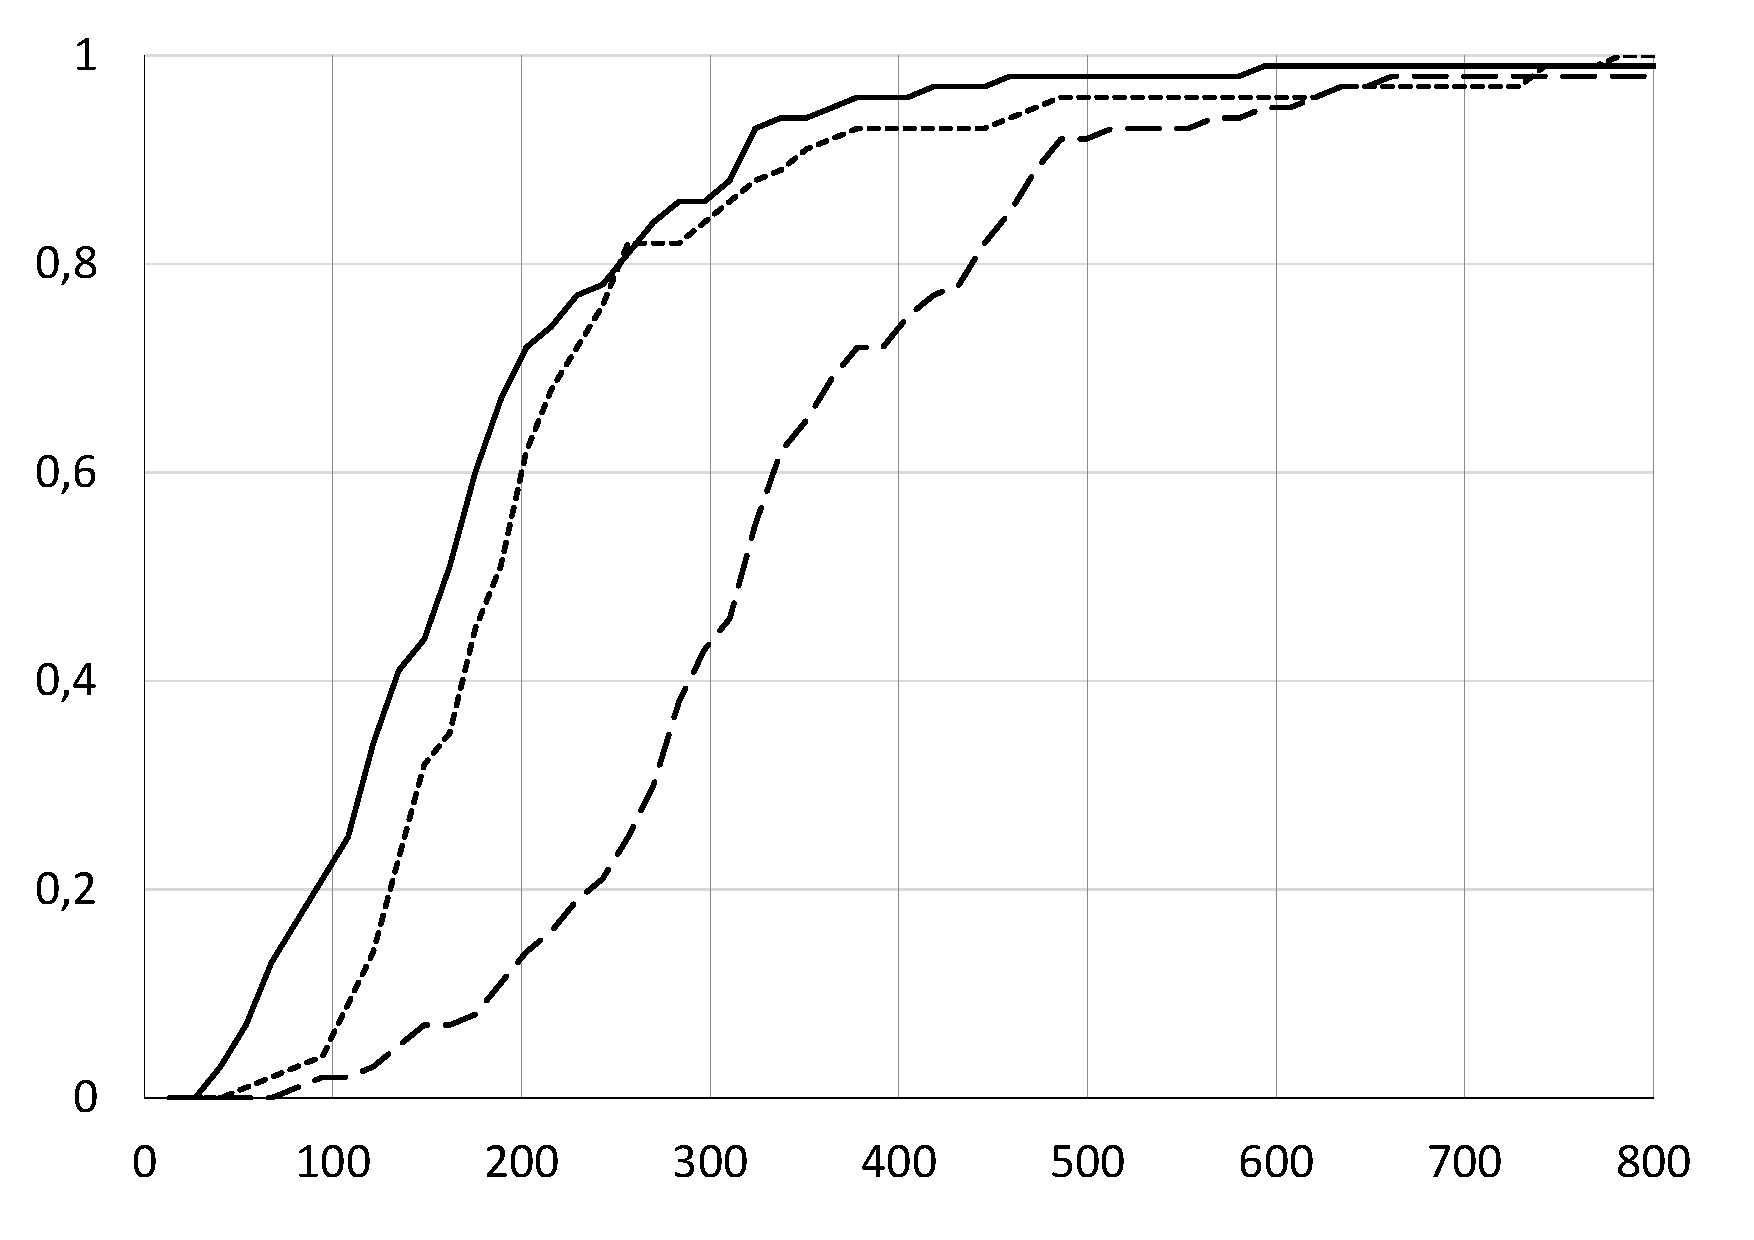
\includegraphics[width=0.50\textwidth]{2D.pdf}
\caption{Operating characteristics using $F_{gr}$ class} 
\label{fig1}
\end{figure}

\begin{figure}
\begin{minipage}{0.5\linewidth}
\center{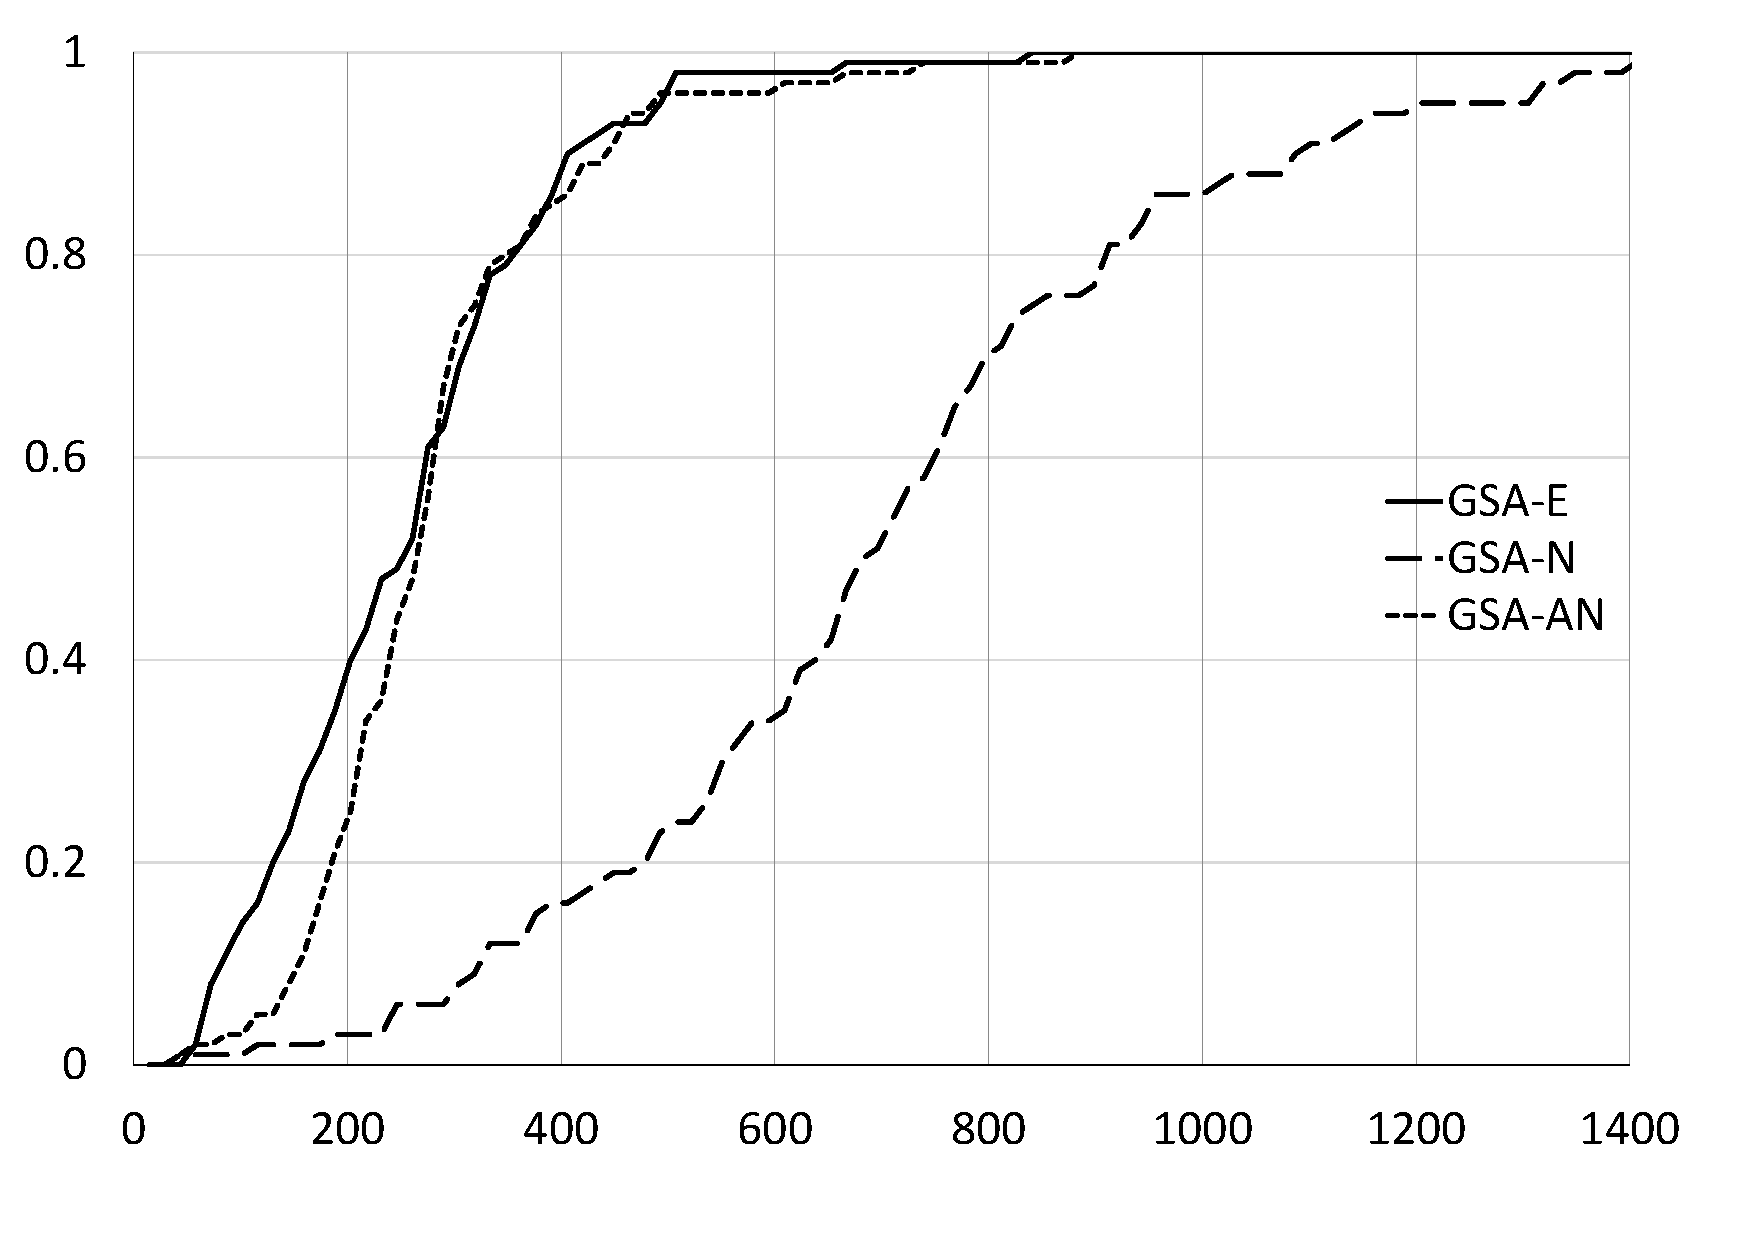
\includegraphics[width=1.0\linewidth]{2DSimple.pdf} \\ (a)}
\end{minipage}
\begin{minipage}{0.5\linewidth}
\center{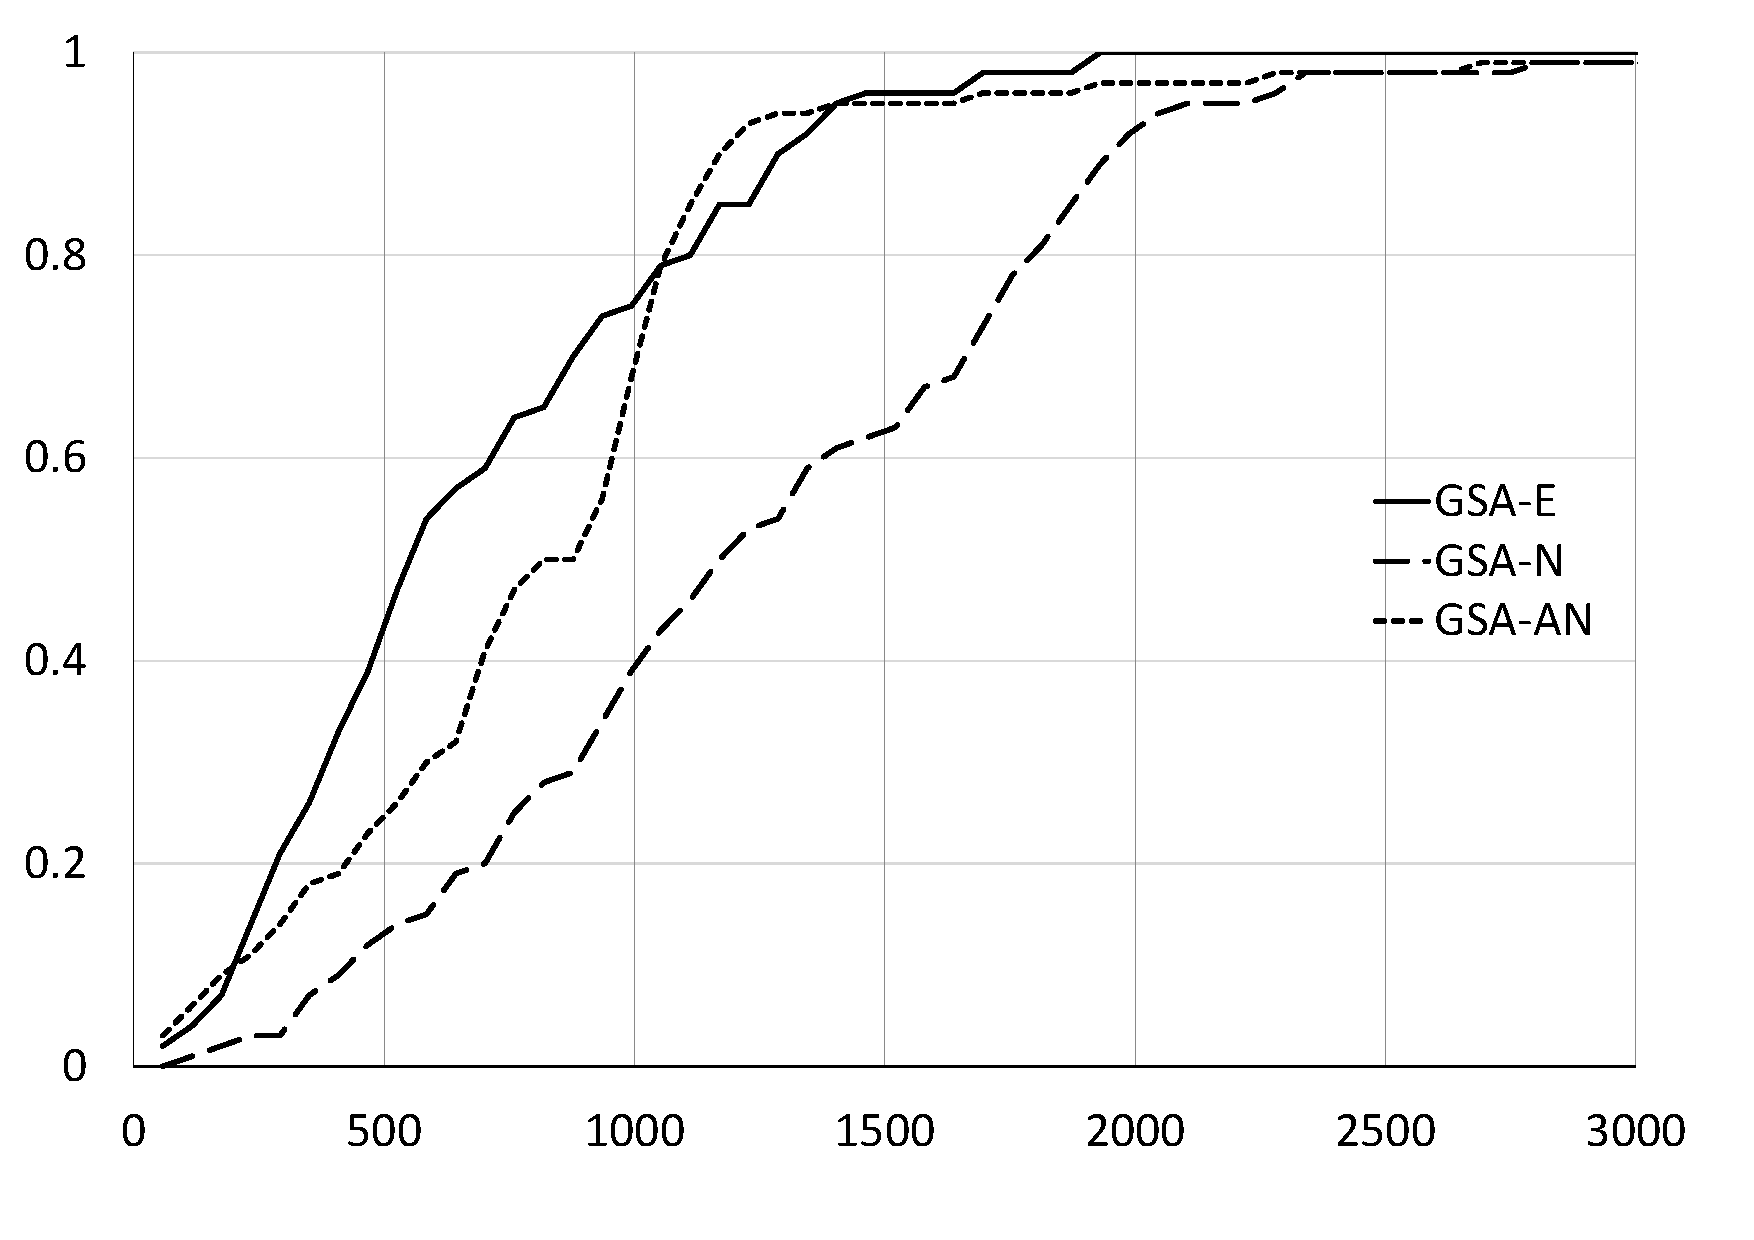
\includegraphics[width=1.0\linewidth]{2DHard.pdf} \\ (b)}
\end{minipage}
\caption{Operating characteristics using 2d GKLS \textit{Simple} (a) and GKLS \textit{Hard} (b) classes}
\label{fig2}
\end{figure}

Вторая серия экспериментов была проведена на четырехмерных задачах классов GKLS \textit{Simple}, GKLS \textit{Hard} (100 функций каждого класса). В Table~\ref{tab2}  представлено среднее число испытаний, выполненных GSA с использованием evolvents ($K_e$), adaptive nested optimization scheme ($K_a$ ), block adaptive nested optimization scheme ($K_ba$). 
На Fig.~\ref{fig3}(a,b) приведены operational characteristics алгоритмов, полученные на классах GKLS \textit{Simple}, GKLS \textit{Hard} соответственно. Непрерывная линия соответсвует алгоритму с использованием evolvents, короткий пунктир -- adaptive nested optimization scheme, длинный пунктир -- block adaptive nested optimization scheme. 
Результаты экспериментов показывают,

\begin{table}
\centering
\caption{Average number of iterations for 4D problems.}\label{tab2}
\begin{tabular}{lcc}
\hline\noalign{\smallskip}
 &    GKLS \textit{Simple} &  GKLS \textit{Hard} \\
\noalign{\smallskip}\hline\noalign{\smallskip}
 $K_e$  &        &       \\
 $K_a$  &  21747 & 35633 \\
 $K_ba$ &  15942 & 33206 \\
\noalign{\smallskip}\hline
\end{tabular}
\end{table}

\begin{figure}
\begin{minipage}{0.5\linewidth}
\center{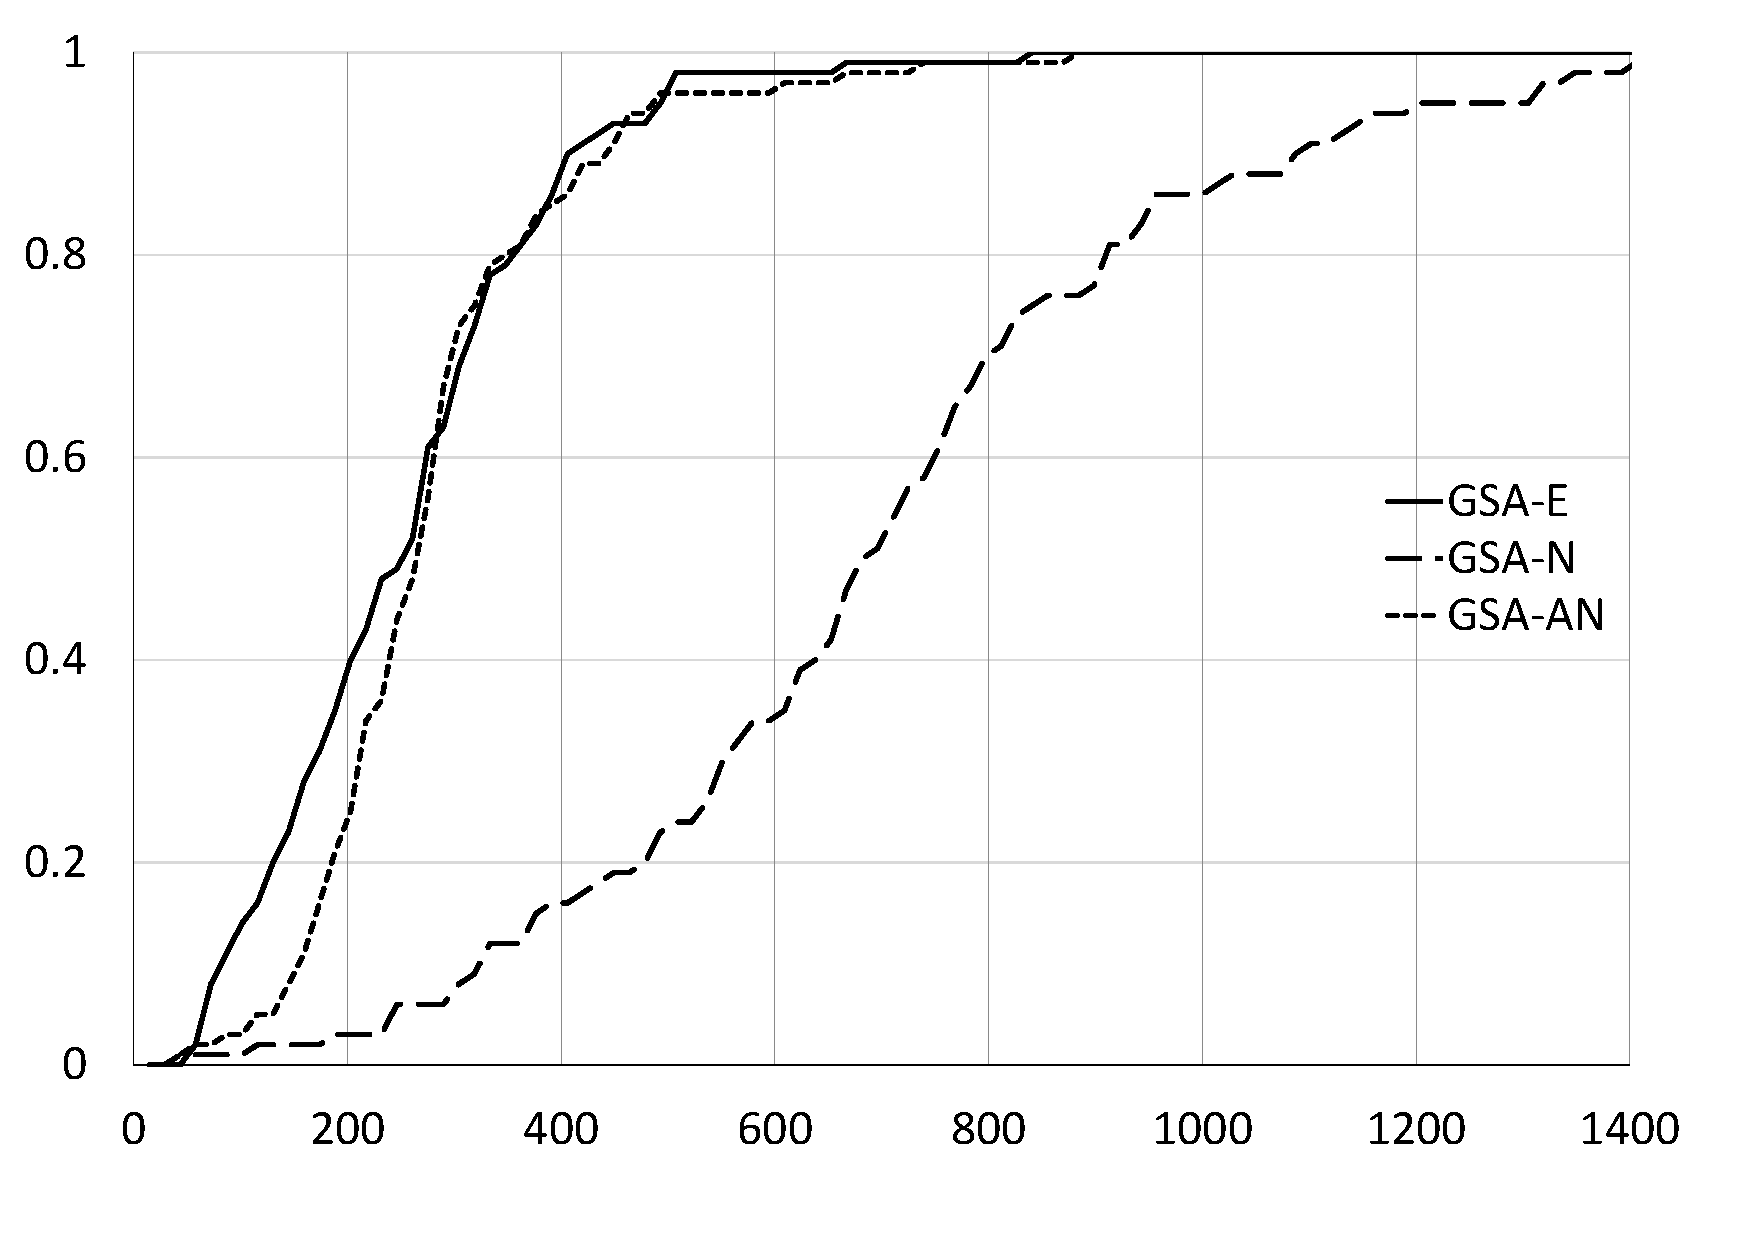
\includegraphics[width=1.0\linewidth]{2DSimple.pdf} \\ (a)}
\end{minipage}
\begin{minipage}{0.5\linewidth}
\center{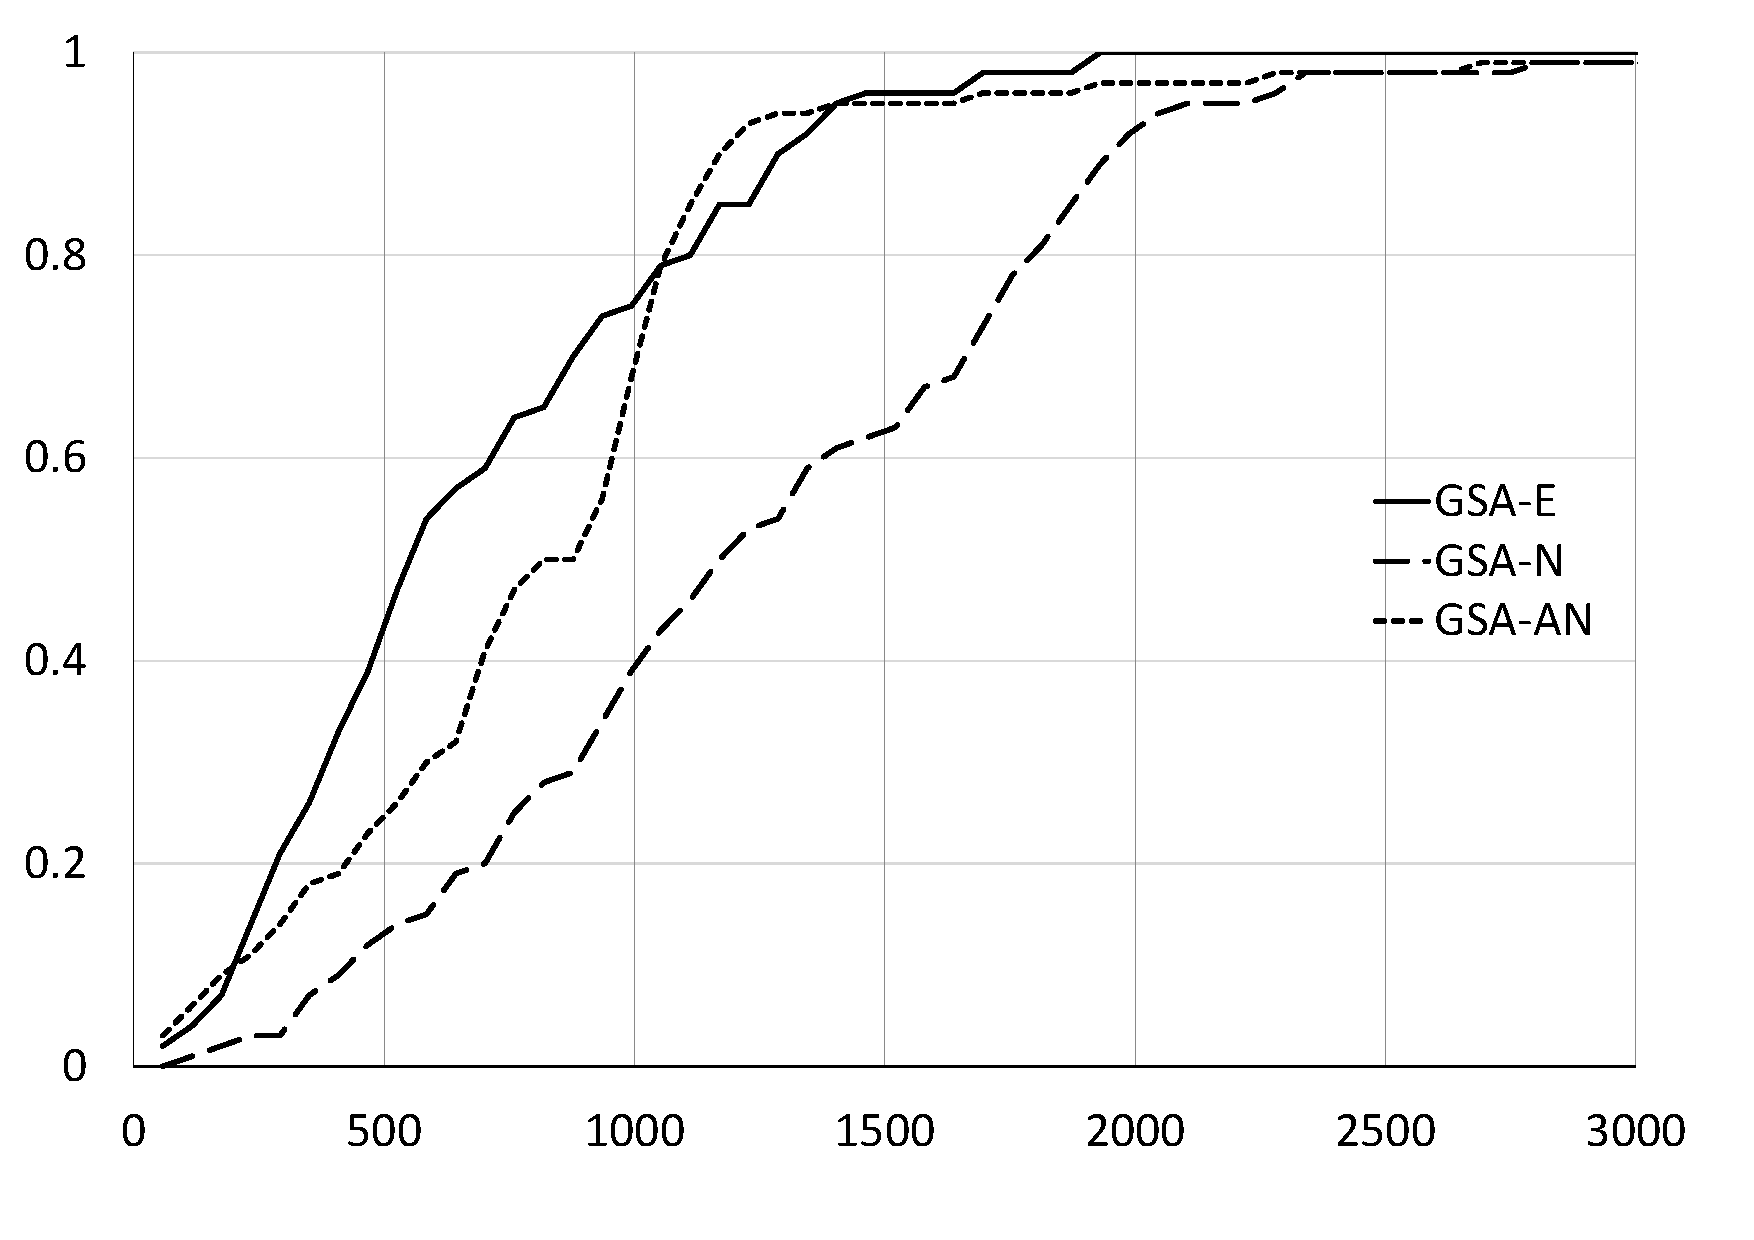
\includegraphics[width=1.0\linewidth]{2DHard.pdf} \\ (b)}
\end{minipage}
\caption{Operating characteristics using 4d GKLS \textit{Simple} (a) and GKLS \textit{Hard} (b) classes}
\label{fig3}
\end{figure}



\section{Conclusion}

В данной работе предложена обобщенная адаптивная схема редукции размерности для задач глобальной оптимизации, комбинирующая использование кривых Пеано и схему вложенной оптимизации. Для решения редуцированных подзадач меньшей размерности используется алгоритм глобального поиска. Приведена вычислительная схема алгоритма, рассмотрены алгоритмические моменты работы адаптивной схемы редукции размерности.
Проведены вычислительные эксперименты на серии тестовых задач с целью сравнения эффективности различных схем редукции размерности. 
Результаты экспериментов показывают, что . 
Перспективы ...


%
% ---- Bibliography ----
%
% BibTeX users should specify bibliography style 'splncs04'.
% References will then be sorted and formatted in the correct style.
%
 \bibliographystyle{splncs04}
 \bibliography{bibliography}


\end{document}
